\section{Background and Related Works}
\label{sec:background}

We introduce %OIDC \cite{OpenIDConnect}, to describe
typical SSO login flows, and discuss existing privacy-preserving solutions and other related works.

\subsection{OpenID Connect and SSO Services}
\label{subsec:OIDC}
OIDC is one of the most popular SSO protocols.
Users and RPs initially register at an IdP with their identities
and other information such as user credentials (e.g., passwords)
and RP endpoints (i.e., the URLs to receive tokens).
It supports three types of login flows, i.e. implicit flow, authorization code flow, and hybrid flow (a mix-up of the other two).
%In the implicit flow, an {\em id token} is generated as the identity token, which contains a user identifier, an RP identifier, the issuer (i.e., IdP), the validity period, and other requested attributes. The IdP signs the id token using its private key to ensure integrity, and sends it to the RP through the user.
%In the authorization code flow, the IdP binds an authorization code with the RP, and sends it to the RP through the user; then, the RP establishes an HTTPS connection to the IdP and uses the authorization code with the RP's credential to obtain the user's identifier and other attributes.
%UPPRESSO is compatible with all three flows.
They work with different steps to request/receive identity tokens, but share the common security requirements of identity tokens.
Next, we focus on the implicit flow to present our designs. In Section \ref{sec:discussion} we discuss the supports for the authorization code flow.

\begin{figure}[t]
  \centering
  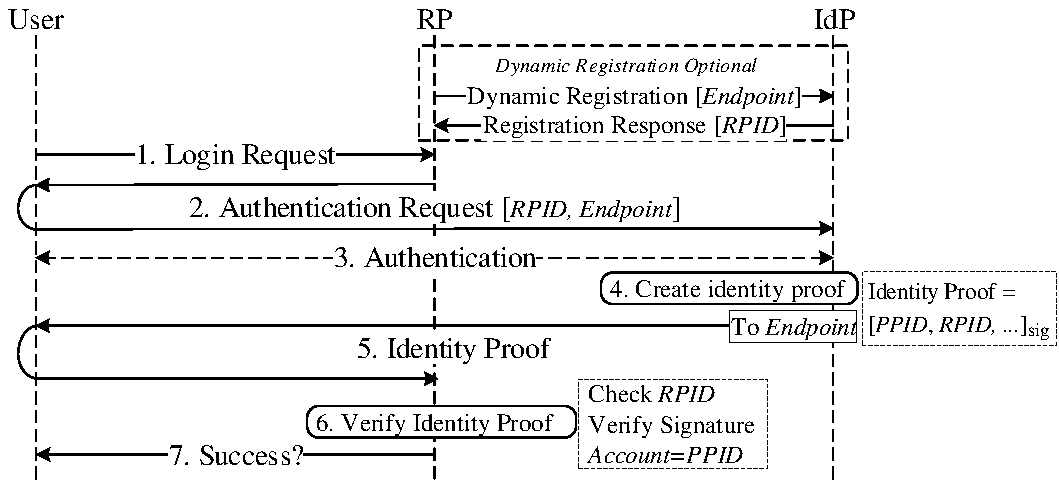
\includegraphics[width=0.9\linewidth]{fig/OIDC1.pdf}
  \caption{The implicit SSO login flow of OIDC.}
  \label{fig:OpenID}
\end{figure}

As shown in Figure \ref{fig:OpenID}, when a user initiates a login request to an RP, the RP constructs an identity-token request with its own identity and the scope of the requested user attributes.
This request is redirected to a trusted IdP.
After authenticating the user, the IdP issues an identity token that will be forwarded by the user to the RP's endpoint.
The token contains the identities (or pseudo-identities) of user and RP,
        a validity period, the requested user attributes, etc.
Finally, the RP verifies the received identity token and allows the user to login as the  enclosed (pseudo-)identity.
The user's operations including redirection, authorization, and forwarding are implemented in user agents (e.g., a browser for web applications).

%Before issuing the identity token,
%    the IdP obtains the user's authorization to enclose the requested attributes.
 %   which are maintained at the IdP by the user.
%The IdP is also a web service.
%The identity token is usually signed by the IdP,
%    and transmitted through secure channels such as TLS/HTTPS.

%extracts user's identifier and returns the authentication result to the user (Step 7).


\begin{table*}[tb]
\footnotesize
    \caption{Privacy-Preserving Solutions of SSO and Identity Federation.}
    \centering
    \begin{tabular}{|c|c|c|c|c|c|c|}
  \hline
  \multirow{3}*{\textbf{~~Solution~~}} &
  \multicolumn{3}{c|}{\textbf{SSO Feature} - supported $\CIRCLE$, unsupported $\Circle$, or partially $\LEFTcircle$} & \multicolumn{3}{c|}{\textbf{Privacy Threat} - prevented $\CIRCLE$, or not $\Circle$} \\ \cline{2-7}
  & User Identity & User Authentication & IdP-Confirmed Selective  & IdP-based & RP-based & Collusive Attack \\
  & at an RP & to Only an IdP &  Attribute Provision & Login Tracing & Identity Linkage & by the IdP and RPs \\\hline\hline
  OIDC w/ PPID \cite{NIST2017draft} & $\CIRCLE$ & $\CIRCLE$ & $\CIRCLE$ & $\Circle$ & $\CIRCLE$ & - \\ \hline
  BrowserID \cite{BrowserID} & $\CIRCLE$ & $\CIRCLE$$^1$ & $\Circle$ & $\CIRCLE$ & $\Circle$ & - \\ \hline
  SPRESSO \cite{SPRESSO} & $\CIRCLE$ & $\CIRCLE$ & $\LEFTcircle$$^2$ & $\CIRCLE$ & $\Circle$ & - \\ \hline  \hline
  PRIMA \cite{prima} & $\CIRCLE$ & $\Circle$ & $\CIRCLE$ & $\CIRCLE$ & $\Circle$ & - \\ \hline
  PseudoID \cite{PseudoID} & $\CIRCLE$ & $\Circle$ & $\LEFTcircle$$^3$ & $\CIRCLE$ & $\CIRCLE$ & $\CIRCLE$ \\ \hline
  EL PASSO \cite{ELPASSO} & $\CIRCLE$ & $\Circle$ & $\CIRCLE$ & $\CIRCLE$ & $\CIRCLE$ & $\CIRCLE$ \\ \hline
  UnlimitID \cite{UnlimitID} & $\CIRCLE$ & $\Circle$ & $\CIRCLE$ & $\CIRCLE$ & $\CIRCLE$ & $\CIRCLE$ \\ \hline
  Opaak \cite{Opaak} & $\LEFTcircle$$^4$ & $\Circle$ & $\Circle$ & $\CIRCLE$ & $\CIRCLE$ & $\CIRCLE$ \\ \hline
  Fabric Idemix \cite{hyperledge-idemix} & $\Circle$$^5$ & $\Circle$ & $\CIRCLE$ & $\CIRCLE$ & $\CIRCLE$ & $\CIRCLE$ \\ \hline
  U-Prove \cite{uprov} & $\CIRCLE$ & $\Circle$ & $\LEFTcircle$$^6$ & $\CIRCLE$ & $\CIRCLE$ & $\CIRCLE$ \\ \hline\hline
  UPPRESSO & $\CIRCLE$ & $\CIRCLE$ & $\CIRCLE$ & $\CIRCLE$ & $\CIRCLE$ & $\Circle$ \\ \hline
\end{tabular}
    \label{tbl:comparison-protocol}
\flushleft
{\footnotesize
1. A BrowserID user generates an \emph{ephemeral} private key to sign the ``subsidiary'' token,
 which is verified by the RP.\\
2. SPRESSO can be extended to provide user attributes in the tokens, while the prototype does not implement this feature.\\
3. Blindly-signed user attributes can be selectively provided using zero-knowledge proofs,
    but not implemented in the prototype.\\
4. Opaak supports exclusive pseudonym options: (\emph{a}) linkable within an RP but unlinkable across multiple RPs and (\emph{b}) unlinkability for any two actions.\\
5. In the original design of Idemix \cite{idemix}, every user logins to an RP with a unique account, but Fabric Idemix implements completely-anonymous services.\\
6. A U-Prove token may contain some attributes \emph{invisible} to the IdP, in addition the ones confirmed by the IdP.}
\end{table*}

Three features are desired in SSO, supported by popular SSO systems \cite{NIST2017draft,OpenIDConnect,rfc6749,SAML,SAMLIdentifier}.

\noindent \textbf{User identification at an RP.}
An RP recognizes each user, as an identity or account \emph{unique}  at the RP,
    and then provides customized services across multiple logins.
%The identity tokens facilitate the target RP to identify each user as a unique account at this RP and this account links the user's multiple login instances to this RP for customized services.

%On the contrary, in anonymous SSO systems \cite{WangWS13,HanCSTW18,HanCSTWW20}
%        the RP only verifies whether he is a legitimate user authenticated by the IdP
%            and receives no information to distinguish every user.

\noindent\textbf{User authentication to {\em only} an IdP.}
%A widely-adopted SSO protocol  usually does not include authentication steps.
The authentication between a user and an IdP is usually conducted \emph{independently}
    of the specifications of widely-adopted SSO protocols \cite{OpenIDConnect,rfc6749,SAML},
where RPs verify only the tokens issued by the IdP.
This brings advantages. First, the IdP authenticates users by any appropriate means (e.g., password,
one-time password, or multi-factor authentication).
%It eliminates the authentication steps between users and an RP,
Meanwhile, a user only maintains his credential at the IdP.
 If it is lost or leaked, the user only renews it at the IdP.
However, if a user proves some \emph{non-ephemeral secret} to RPs, which is valid across multiple login instances (i.e., authentication steps are actually involved),
 he has to notify each RP when lost or leaked, %during its validity period,
  or additional revocation checking is needed \cite{ELPASSO,UnlimitID}.

%. %(or even the user logins from another computer).

\noindent\textbf{Selective IdP-confirmed attribute provision.}
An IdP usually provides user attributes in the tokens \cite{OpenIDConnect,rfc6749}, in addition to user (pseudo-)identities.
These attributes are maintained by users at a trusted IdP.
%    for example,
%        when Facebook provides social networking services,
%         it also issues identity tokens enclosing user identities and various attributes.
Before enclosing any attributes in a token, the IdP obtains a user's authorization or provides only attributes pre-selected by the user.
%So no distinctive attributes such as telephone number and Email address are enclosed in the identity tokens of privacy-preserving SSO systems.

%\vspace{1mm}
%\noindent\textbf{RP Dynamic Registration.}
%In addition to manual registrations,
%    OIDC also supports dynamic registrations
%    for an RP to register by online means \cite{DynamicRegistration}.
%The (unregistered) RP sends a registration request
%        with endpoints to receive identity tokens (and other information),
%        to the IdP.
%After a successful registration,
% the IdP assigns a unique RP identity in the response.
%

%UPPRESSO leverages this function and slightly modifies the dynamic registration process to implement the {\em $PID_{RP}$ registration} process (see details in Section \ref{sec:UPPRESSO}.C), which allows an RP to generate different privacy-preserving RP identifiers and register them with the IdP.


\subsection{Privacy-Preserving SSO and Identity Federation}
\label{subsec-solutions}

We summarize existing privacy-preserving solutions for SSO and identity federation in Table \ref{tbl:comparison-protocol}.
Widely-adopted SSO protocols \cite{OpenIDConnect,rfc6749,SAML,SAMLIdentifier} allow a user to login to an RP
%    after being authenticated by the IdP,
\emph{without holding any permanent secret verified by the RP or by himself maintaining an account at the RP}.
While providing these convenient features, existing privacy-preserving SSO approaches \cite{BrowserID,SPRESSO,NIST2017draft} prevent either the IdP-based login tracing or the RP-based identity linkage, and UPPRESSO prevents both of them.

Identity federation enables a user registered at a trusted IdP to be accepted by other parties,
            with different accounts sometimes,
        but \emph{more user operations} are involved than those of SSO.
Privacy-preserving identity federation
    protects user privacy against even collusive attacks by the IdP and RPs,
    but requires a user \cite{ELPASSO,UnlimitID,hyperledge-idemix,PseudoID,Opaak,uprov} to (\emph{a}) \emph{hold long-term secrets verified by RPs},
            in addition to the authentication credentials for the IdP,
                and (\emph{b}) \emph{locally manage the accounts at different RPs}.
That is, there are actually some authentication steps between a user and RPs (called asynchronous authentication \cite{ELPASSO}).

Pairwise pseudonymous identifiers (PPIDs) are specified in SSO protocols \cite{OpenIDConnect, SAMLIdentifier} and recommended \cite{NIST2017draft}
to protect user privacy against curious RPs.
When issuing an identity token,
        an IdP encloses a user PPID (but not the identity at the IdP).
Given a user, the IdP assigns a unique PPID based on the target RP.
So colluding RPs cannot link the user identities (or accounts).
PPIDs cannot prevent the IdP-based login tracing because the IdP needs the RP's identity to issue tokens.



Several solutions prevent the IdP-based login tracing but are vulnerable to the RP-based identity linkage.
In BrowserID \cite{BrowserID} (formerly known as Firefox Accounts \cite{FirefoxAccount} and Mozilla Persona \cite{persona}), an IdP %(called the primary identity authority in BrowserID)
issues a special token (called user certificate) to bind a user identity to an ephemeral public key.
With the corresponding private key, the user signs a ``subsidiary'' token (called identity assertion) to bind the target RP's identity and sends both tokens to the RP.
In SPRESSO \cite{SPRESSO} an RP creates a verifiable one-time pseudo-identity for itself in each login, which is enclosed in the identity token issued by an IdP. %and the user identity.
A PRIMA IdP signs a credential
%\footnote{For the message signed by the IdP works with a user secret verified by an RP,
%    it is usually called a credential  in identity federation instead of token.}
 binding a verification key and user attributes \cite{prima},
  where the key is considered as the user identity.
The user selectively provides IdP-confirmed attributes to an RP using his signing key \cite{Oblivion}.
In these schemes \cite{BrowserID,SPRESSO,prima}, colluding RPs could link a user based on his unique identity in the tokens (or credentials).


PseudoID \cite{PseudoID} introduces another independent service in addition to an IdP to \emph{blindly} sign \cite{blind-sign}
    an access token binding a pseudonym and a user secret.
Then, the user unblinds this token and the IdP will assert it,
    which allows the user to login to an RP using his secret.
Two kinds of privacy threats are prevented, because (\emph{a}) the RP's identity is not enclosed in the tokens
    and (\emph{b}) the user selects different pseudonyms when visiting RPs.
Collusive attacks by the IdP and RPs are also prevented,
    for they cannot link two blindly-signed tokens.

% the user must use the secret to login to RP, because no RP identity is enclosed in the token.


%However, the user has to permanently keep the secret preimage for each account in an RP.

In EL PASSO \cite{ELPASSO}, after authenticating a user,
    an IdP signs an \emph{anonymous credential} \cite{anon-credential} binding a secret,
         both of which are securely kept on the user's device.
When attempting to login to an RP,
    the user proves that he is the owner of this credential using the secret,
        and discloses selective attributes in the credential.
Although one credential is proved to multiple RPs,
        \emph{user-managed pseudonyms} and \emph{anonymous credentials} prevent the RPs, even when collusive with the IdP, from linking the users across the RPs.
UnlimitID \cite{UnlimitID} presents similar designs based on anonymous credentials \cite{anon-credential},
        to prevent collusive attacks by the IdP and RPs.
NEXTLEAP \cite{nextleap} builds anonymous secure messaging on top of UnlimitID.

%    but a user has to by himself manage pseudonyms for different RPs.
%For example,
%    the RP domain (e.g., \verb+www.RP.com+) is used as a factor to locally generate the user's account (or pseudonym) at this RP.

Anonymous credentials \cite{anon-credential-2001,anon-credential} are used in more flexible ways.
Opaak \cite{Opaak} keeps IdP-signed anonymous credentials %in mobile phones
 as pseudonym tokens,
    which bind a user's secret key.
Idemix anonymous credentials \cite{idemix}
 are integrated in Hyperledger Fabric \cite{hyperledge-idemix} to implement completely-unlinkable pseudonyms
        and IdP-confirmed selective attribute disclosure.
With a U-Prove token \cite{uprov,uprove-conference} from an IdP,
    a user is enabled to authenticate himself to an RP and selectively disclose attributes.

